% LaTeX rebuttal letter example. 
% 
% Copyright 2019 Friedemann Zenke, fzenke.net
%
% Based on examples by Dirk Eddelbuettel, Fran and others from 
% https://tex.stackexchange.com/questions/2317/latex-style-or-macro-for-detailed-response-to-referee-report
% 
% Licensed under cc by-sa 3.0 with attribution required.
% See https://creativecommons.org/licenses/by-sa/3.0/
% and https://stackoverflow.blog/2009/06/25/attribution-required/

\documentclass[11pt]{article}
\usepackage[utf8]{inputenc}
\usepackage{fullpage}
\usepackage{amsfonts}
\usepackage{amsmath}
\usepackage{bm}
\usepackage{xcolor}
\usepackage{changepage}
% import Eq and Section references from the main manuscript where needed
% \usepackage{xr}
% \externaldocument{manuscript}
\usepackage{array}
\usepackage{multirow}
\newcolumntype{A}{>{\color{blue}\arraybackslash}m{3em}}
\newcolumntype{B}{>{\color{blue}\centering\arraybackslash}m{1em}}
\newcolumntype{C}{>{\color{blue}\centering\arraybackslash}m{2em}}
\newcolumntype{D}{>{\color{blue}\centering\arraybackslash}m{5.5em}}
\newcolumntype{E}{>{\color{blue}\arraybackslash}m{21em}}
\newcolumntype{F}{>{\color{blue}\arraybackslash}m{0.95\columnwidth}}
\renewcommand{\thetable}{\Roman{table}}
\usepackage{subcaption}
% package needed for optional arguments
\usepackage{xifthen}
% define counters for reviewers and their points
\newcounter{reviewer}
\setcounter{reviewer}{0}
\newcounter{point}[reviewer]
\setcounter{point}{0}
\newcounter{suggestion}
\setcounter{suggestion}{0}

% This refines the format of how the reviewer/point reference will appear.
\renewcommand{\thepoint}{P\,\thereviewer.\arabic{point}} 
\renewcommand{\thesuggestion}{\arabic{suggestion}} 

% command declarations for reviewer points and our responses
\newcommand{\reviewersection}{\stepcounter{reviewer} \bigskip \hrule
                  \section*{Reviewer \thereviewer}}

\newenvironment{point}
   {\refstepcounter{point} \bigskip \noindent {\textbf{Reviewer~Point~\thepoint} } ---\ }
   {\par }

\newcommand{\shortpoint}[1]{\refstepcounter{point}  \bigskip \noindent 
	{\textbf{Reviewer~Point~\thepoint} } ---~#1\par }

\newenvironment{reply}
   {\medskip \noindent \begin{sf}\textbf{Reply}: \  }
   {\medskip \end{sf}}

\newcommand{\shortreply}[2][]{\medskip \noindent \begin{sf}\textbf{Reply}:\  #2
	\ifthenelse{\equal{#1}{}}{}{ \hfill \footnotesize (#1)}%
	\medskip \end{sf}}

\newenvironment{suggestion}
   {\refstepcounter{suggestion} \bigskip \noindent {\textbf{Suggestion~\thesuggestion} } ---\ }
   {\par }

\usepackage{tabularx,ragged2e,caption}
\usepackage[colorinlistoftodos]{todonotes}
\newcommand{\rv}[1]{\textcolor{red}{#1}}
\newcommand{\rp}[1]{\textcolor{purple}{#1}}
\newcommand{\xt}[1]{\textcolor{blue}{#1}}
\newcommand{\zj}[1]{\textcolor{green}{#1}}
\usepackage{booktabs}
\usepackage[style=ieee,sorting=none,backend=bibtex]{biblatex}
\addbibresource{./ref.bib}

\begin{document}

\section*{Summary of changes}
% General intro text goes here
We really appreciate the valuable and critical comments on our work by the reviewers. 
Having studied the comments carefully, we have made considerable modifications to the revised manuscript. In the following, we address their concerns point by point. We also uploaded another version of the manuscript with highlighted texts corresponding to the new changes. Please look for the highlighted changes \xt{(in blue)} mentioned in the following summary in this annotated version. The modified or added texts are also included wherever possible in the response to each comment below.

% Let's start point-by-point with Reviewer 1
% \reviewersection

\subsection*{Associate Editor}
The manuscript introduces DDBot, a framework leveraging differentiable physics simulators and gradient‐based optimization for robotic excavation in unknown granular materials, incorporating regularization techniques to mitigate gradient explosion during skill parameter learning. Three reviewers reviewed the paper and have identified critical comments that need to be addressed, among them:

\begin{reply}
\rp{Dear editor, we are very grateful for the valuable comments given by you and the reviewers. Please read the following responses to each comment.}

\vspace{0.3cm}\noindent\rv{\textbf{- The manuscript fails to summarize its core contributions, instead reading like a collection of related works without highlighting what is truly new (Reviewer 1).}}

\begin{adjustwidth}{20pt}{20pt}
\noindent\rp{Thanks for the insightful comment. We have made significant modifications in the abstract, introduction and conclusion sections to better reflect the core contributions of this article. They are quoted as follows.}

\vspace{0.3cm}\noindent\xt{\textbf{Abstract} (Page 1)}

Automating the manipulation of granular materials poses significant challenges due to complex contact dynamics, unpredictable material properties, and intricate system states. Existing approaches often fail to achieve efficiency and accuracy in such tasks. To fill the research gap, this paper \xt{studies the small-scale and high-precision granular material digging task with unknown physical properties. A new framework, named differentiable digging robot (DDBot), is proposed to manipulate granular materials, including sand and soil.}

\xt{Specifically, we equip DDBot with a differentiable physics-based simulator, tailored for granular material manipulation, powered by GPU-accelerated parallel computing and automatic differentiation. DDBot can perform efficient differentiable system identification and high-precision digging skill optimisation for unknown granular materials, which is enabled by a differentiable skill-to-action mapping, a task-oriented demonstration method, gradient clipping and line search-based gradient descent.}

\xt{Experimental results show that DDBot can efficiently (converge within $5$ to $20$ minutes) identify unknown granular material dynamics and optimise digging skills, with high-precision results in zero-shot real-world deployments, highlighting its practicality. Benchmark results against state-of-the-art baselines also confirm the robustness and efficiency of DDBot in such digging tasks.}

\vspace{0.3cm}\noindent\xt{\textbf{Introduction} (Page 2, left column, paragraphs 2 to 4)}

\xt{...}

\xt{To fill the research gap, this article makes the following contributions to the robotisation of real-world, small-scale and high-precision granular material digging tasks with unknown material properties.}

\xt{First, to the best of our knowledge, this is the first attempt to develop an efficient and high-fidelity differentiable simulator specifically designed for granular material manipulation. It supports efficient forward dynamics computation to train data-driven methods, such as DRL, and evaluate non-learning methods, such as MPC. It also enables efficient automatic differentiation to support gradient-based optimisation methods, such as RMSProp~\cite{tieleman2012rmsprop}.}

\xt{Secondly, based on the proposed simulator, we present a novel framework, named differentiable digging robot (DDBot) (Figure 1), which allows first-order gradient-based optimisation in system identification tasks and small-scale high-precision digging tasks for real-world granular materials with unknown properties. We experimentally show that gradient-clipping is effective in stopping gradient explosion in SVK and DP-based granular dynamics.} 

\xt{DDBot uses a differentiable digging skill to significantly reduce the solution space and improve manipulation quality, initialises manipulation solution before optimisation via target-oriented demonstrations to accelerate convergence, and performs line search-based gradient descent with adaptive step sizes to stabilise convergence.}

\xt{Last, we experimentally confirm the feasibility of differentiable system identification with soil and sand materials. For digging skill optimisation, we evaluate and benchmark, for the first time, the performances on a series of soil and sand digging tasks with state-of-the-art manipulation optimisation methods, confirming the robustness and efficiency of our DDBot system. Evaluation on a real-world UR5 robot arm is performed to confirm the practicality of the optimised digging motions.}

\xt{...}

\vspace{0.3cm}\noindent\xt{\textbf{Conclusions} (Page 16)}

\xt{Granular material manipulation is of high importance to many real-world scenarios, but the field significantly lacks research and engineering experiences, particularly in small-scale and high-precision manipulation tasks with unknown material properties.} This work thereby studied the challenging real-world granular material manipulation problem with unknown material properties in the context of \textit{small-scale and high-precision} digging. \xt{A differentiable digging robot (DDBot) system was developed for solving such manipulation tasks using a differentiable physics (DP) simulator and a first-order gradient-based optimisation method (RMSProp). The DP simulator was tailored for granular material manipulation for fast data collection, trajectory evaluation and gradient computation, powered by GPU-accelerated parallel computing and automatic differentiation. A differentiable digging skill was designed to reduce the solution space and improve manipulation motion quality. The issues of exploding and fluctuating gradients were studied and resolved through gradient clipping and line search, enabling gradient-based optimisation. To speed up convergence, a digging target-oriented demonstration method is created to serve as an initial solution or form an explorative data distribution.}

\xt{The quantitative and visualisation results of extensive experiments confirmed that DDBot achieves high-quality system identification and skill optimisation performances with sand and soil materials. The optimised solutions were successfully deployed on a UR5e robotic arm in the real world without any adaptation (zero-shot sim-to-real transfer), achieving high digging precision (location and depth errors $<6$ mm, area error $\sim10.8$ cm$^2$). In addition, with GPU acceleration and the proposed gradient treatments, DDBot achieved nearly practically applicable optimisation efficiency (converges in $5$ minutes with a good initial solution).} 

\xt{The performance of DDBot was benchmarked against gradient-based trajectory optimisation, deep reinforcement learning (PointNet-backboned goal-conditioned soft actor-critic) and model predictive control (covariance matrix adaptation map-annealing). Results showed that trajectory optimisation and reinforcement learning (RL) failed in all tasks, while our method and model predictive control succeeded with comparable performances and efficiency. It was suggested that 1) optimisation in the trajectory space for long-horizon tasks should be avoided whenever possible, and 2) when an efficient and physically realistic simulator is available, DRL methods that learn a neural network are counterproductive, gradient-free methods like CMA-MAE lack considerations of the system dynamics, whereas first-order gradient descent methods are preferred for optimisation in the skill parameter space leveraging the gradients computed through the system dynamics.}

\xt{...}

\end{adjustwidth}

\vspace{0.3cm}\noindent\rv{\textbf{- The theoretical innovation is questioned, as the approach largely applies existing regularization techniques without clear advancement over prior art (Reviewer 11).}}
\begin{adjustwidth}{20pt}{20pt}
\rp{Thanks for the important comment regarding the novelty of the article. We apologise for the confusing wording that was used in the previous manuscript. We agree that the gradient regularisation techniques themselves have been adopted in other research and engineering practices for decades. However, their effectiveness has not been studied in the context of differentiable physics simulation, especially not for granular material manipulation tasks modelled by the St. Venant-Kirchoff (SVK) elastic energy and the Drucker-Prager (DP) plastic yield criterion. We have made modifications to highlight the experimental novelty in the investigation of the gradient instability issues and the effects of the techniques, instead of their theoretical development. Below are the key relevant changes.}

\vspace{0.3cm}\noindent\xt{\textbf{Introduction} (Page 2, left column, paragraphs 2 to 4)}

\xt{...}

\xt{... We experimentally show that gradient-clipping is effective in stopping gradient explosion in SVK and DP-based granular dynamics...}

\xt{...}

\vspace{0.3cm}\noindent\xt{\textbf{Method} (Section III-E, Page 8, left column, last paragraph)}

\xt{...}

We \xt{experiment on} three techniques to regularise the scale of the gradient for key variables in the MLS-MPM algorithm, namely \textit{clipping, dynamic-scaling, and normalisation}.

\xt{...}

\vspace{0.3cm}\noindent\xt{\textbf{Conclusions} (Page 16)}

\xt{... The issues of exploding and fluctuating gradients were studied and resolved through gradient clipping and line search, enabling gradient-based optimisation...}

\end{adjustwidth}

\vspace{0.3cm}\noindent\rv{\textbf{- Algorithm 1 is overly long and Algorithm 2 adds little value; both should be consolidated or simplified into a single, clear procedure (Reviewers 2, 11).}}
\begin{adjustwidth}{20pt}{20pt}
\rp{Thanks for pointing out the poor presentation of the algorithms. We have made considerable changes in section III-D to provide a clearer picture of the differentiable skill design. In particular, we provide the formal mathematical definitions of the four phases of the digging skill with equations (Eqs. 8 to 22) instead of the original algorithm 1. With the equations, we shrunk the original algorithm 1 significantly (now algorithm 2 in the updated manuscript) to only present the assembly process of the four phases that form an action trajectory. In addition, the original algorithm 2 has been removed. The changes are also quoted below.}

\vspace{0.3cm}\noindent\xt{\textbf{Method} (Section III-B, Page 5)}

\xt{...}

\xt{The skill comprises four phases graphically illustrated by Fig. 2 and mathematically defined by Eqs. 8 to 22, with a list of notations comprised in Table 1. Algorithm 2 presents the assembly of the calculated end-effector displacements into the complete trajectory $\bar{a}(\pmb{\theta})$.}

\begin{table}[h]
\small
\centering
\begin{tabular}{>{\color{blue}}l}
\toprule
\textbf{Algorithm 2}: Skill-to-action mapping $\bar{a}(\pmb{\theta})=\{a_0,..,a_T\}$\\
\midrule
Inputs: $\theta_{ displace},\theta_{ rotate},\theta_{ insert\_dist},\theta_{ push\_dist},\theta_{ push\_angle}$\\
$d_{ lift}, v_l,v_w,\Delta t$. \\
Output: $\bar{a}=\{a_0,a_1,...,a_T\}$\\
\midrule
With Eqs.~\ref{eq:d1} to~\ref{eq:delta_d4}, Compute: \\
$T_1$, $T_2$, $T_3$, $T_4$, $\Delta x_1$, $\Delta rx_1$, $\Delta x_2$, $\Delta z_2$, $\Delta x_3$, $\Delta z_3$, $\Delta rx_4$, $\Delta z_4$\\
Let $T =T_1+T_2+T_3+T_4$\\
For $t$ from $0$ to $T$: \hspace{0.73cm} $a_t = [0.0, 0.0, 0.0, 0.0, 0.0, 0.0]$\\
For $t$ from $0$ to $T_1-1$: \hspace{0.07cm} $a_t[0] = \Delta x_1$, $a_t[3]=\Delta rx_1$\\
For $t$ from $T_1$ to $T_2-1$: $a_t[0] = \Delta x_2$, $a_t[2]=\Delta z_2$\\
For $t$ from $T_2$ to $T_3-1$: $a_t[0] = \Delta x_3$, $a_t[2]=\Delta z_3$\\
For $t$ from $T_3$ to $T_4-1$: $a_t[3] = \Delta rx_4$, $a_t[2]=\Delta z_4$\\
\bottomrule
\end{tabular}
\end{table}

\xt{\textbf{Phase 1:} moving the shovel in the world's $x$ axis by a distance $d_1$ and rotating about the shovel's $x$ axis by an angle $\varphi_1$. Eqs.~\ref{eq:d1} to ~\ref{eq:delta_d1} define the calculation of the actions for phase 1 from $\theta_{displace}$ and $\theta_{rotate}$.}

\setcounter{equation}{7}
\begingroup\makeatletter\def\f@size{8}\check@mathfonts\xt{\vspace{-0.3cm}
\begin{flalign}
    &d_1 = \theta_{displace} \cdot 0.12, &&\varphi_1 = \theta_{rotate} \cdot \pi / 3&&&\label{eq:d1}\\
    &T^{float}_{d_1} = |d_1 / (v_l\cdot\Delta t)|, &&T^{float}_{\varphi_1} = |\varphi_1/(v_w\cdot\Delta t)|&&&\label{eq:Tf1}\\
    &T^{float}_1=max(T^{float}_{d_1}, T^{float}_{\varphi_1}), &&T_1 = round(T^{float}_1)&&&\label{eq:Ti1}\\
    &\Delta x_1 = \begin{cases}
        \frac{d_1}{T_1},\ T_1>0\\
        0,\  T_1=0
        \end{cases}\hspace{-0.4cm},
    &&\Delta rx_1 = \begin{cases}
        \frac{\varphi_1}{T_1},\ T_1>0\\
        0,\  T_1=0
        \end{cases}\label{eq:delta_d1}
\end{flalign}}
\endgroup

\xt{\textbf{Phase 2:} inserting the shovel into the soil/sand by a distance $d_2$ along its pointing direction. Eqs.~\ref{eq:d2} to ~\ref{eq:delta_d2} define the calculation of the actions for phase 2 from $\theta_{rotate}$ and $\theta_{insert\_dist}$.}

\begingroup\makeatletter\def\f@size{8}\check@mathfonts\xt{\vspace{-0.3cm}
\begin{flalign}
    &d_2 = (\theta_{insert\_dist}+1)\cdot0.03,\ \varphi_2 = \varphi_1 + \pi /2 &&\label{eq:d2}\\
    &T^{float}_2 = d_2 / (v_l\cdot\Delta t)\label{eq:Tf2}\\
    &T_2 = round(T^{float}_2)\label{eq:Ti2}\\
    &\Delta x_2 = \begin{cases}
        \frac{d_2 \cdot \cos(\varphi_{2})}{T_2},\ T_2>0\\
        0,\  T_2=0
        \end{cases},\ 
    \Delta z_2 = \begin{cases}
        \frac{-d_2 \cdot \sin(\varphi_{2})}{T_2},\ T_2>0\\
        0,\  T_2=0
        \end{cases}\hspace{-1cm}&&\label{eq:delta_d2}
\end{flalign}}
\endgroup

\xt{\textbf{Phase 3:} pushing towards an angle $\varphi_3$ by a distance $d_3$. Eqs.~\ref{eq:d3} to~\ref{eq:delta_d3} define the calculation of the actions for phase 3 from $\theta_{push\_dist}$ and $\theta_{push\_angle}$}.
\begingroup\makeatletter\def\f@size{8}\check@mathfonts\xt{\vspace{-0.3cm}
\begin{flalign}
    &d_3 = (\theta_{push\_dist} + 1) \cdot 0.1 + 0.04,\ \varphi_3 = (\theta_{push\_angle} + 3) \cdot \pi /3\hspace{-0.4cm}&&\label{eq:d3}\\
    &T^{float}_3 = |d_3 / (v_l\cdot\Delta t)|&&\label{eq:Tf3}\\
    &T_3 = round(T^{float}_3)&&\label{eq:Ti3}\\
    &\Delta x_3 = \begin{cases}
        \frac{d_3 \cdot \cos(\varphi_3)}{T_3},\ T_3>0\\
        0,\  T_3=0
        \end{cases},\
    \Delta z_3 = \begin{cases}
        \frac{d_3 \cdot \sin(\varphi_3)}{T_3},\ T_3>0\\
        0,\  T_3=0
        \end{cases}\hspace{-1cm}&&\label{eq:delta_d3}
\end{flalign}}
\endgroup

\xt{\textbf{Phase 4:} rotating back to straight and lifting for a constant distance $d_4=0.01$ m. Eqs.~\ref{eq:Tf4} to~\ref{eq:delta_d4} define the calculation of actions for phase 4.}
\begingroup\makeatletter\def\f@size{8}\check@mathfonts\xt{\vspace{-0.3cm}
\begin{flalign}
    &T^{float}_{d_4} = d_4 / (v_l\cdot\Delta t) &&&\label{eq:Tf4}\\
    &T^{float}_4 = max(T^{float}_{\varphi_1}, T^{float}_{lift}), &&T_4 = round(T^{float}_4)&&&\label{eq:Ti4}\\
    &\Delta rx_4 = \frac{- \varphi_1}{T_4},&&\Delta z_4 = \frac{d_4}{T_4}&&&\label{eq:delta_d4}
\end{flalign}}
\endgroup

\xt{...}

\end{adjustwidth}

\vspace{0.3cm}\noindent\rv{\textbf{- Critical symbols—such as the $\delta x$, $\delta y$, … action offsets—and functions like dim() appear without definition; a notation table is needed (Reviewers 2, 11).}}

\begin{adjustwidth}{20pt}{20pt}
\rp{Indeed, we have left some symbols undefined in the previous manuscript. Thanks for the careful inspections. We have added a notation table and provide the missing definitions of the undefined symbols. The changes are quoted below.}

\vspace{0.3cm}\noindent\xt{\textbf{Method} (Section III-A, Page 4, right column, paragraph 2)}

\xt{...}

\textbf{Actions:} An action of the robot manipulator at each step here is a 6D displacement vector in the Cartesian space (i.e., end-effector tip frame) $a=[\Delta x, \Delta y, \Delta z, \Delta a, \Delta b, \Delta c]\in\mathcal{A}\subset\mathbb{R}^6$, \rp{i.e., it controls the amount of translational changes in the $x$, $y$, $z$ directions and the rotational changes about these three axes}...

\xt{...}

\clearpage
\vspace{0.3cm}\noindent\xt{\textbf{Method} (Section III-B, Page 6, left column, Table I)}

\begin{table}[h]
\small
\centering
\begin{tabular}{>{\color{blue}}l>{\color{blue}}l}
\toprule
\textbf{Symbol} & \textbf{Meaning} \\
\midrule
$\theta_{\rm displace}$       & parameter: translational displacement in the world's $x$ direction \\
$\theta_{\rm rotate}$         & parameter: rotational displacement about $rx$ (end-effector's $x$ direction) \\
$\theta_{\rm insert\_dist}$   & parameter: insertion distance \\
$\theta_{\rm push\_dist}$     & parameter: pushing distance \\
$\theta_{\rm push\_ang}$      & parameter: pushing angle \\
$d_i$                         & translational displacement in phase $i$ (m) \\
$\varphi_i$                   & rotational displacement in phase $i$ (rad) \\
$v_l$                         & end‐effector linear speed (m/s) \\
$v_w$                         & end‐effector angular speed (rad/s) \\
$\Delta t$                    & simulation time stepsize\\
$T^{float}_i$                 & real‐valued timesteps required in phase $i$\\
$T_{i}$                       & integer timesteps used in phase $i$ \\
$max()$                       & returning the maximal value among the inputs\\
$round()$                     & returning the rounded value of an input\\
$exp()$                       & returning the exponential of the inputs\\
$det()$                       & returning the determinant of the inputs\\
$\Delta x_i,\Delta z_i$       & per‐step translations along $x,z$ axes for phase $i$ (m) \\
$\Delta rx_i$                 & per‐step rotation about $rx$ in phase $i$ (rad) \\
$\bar{a}[i:j]$                & the $i$-th (inclusive) to the $j$-th (exclusive) actions of the skill\\
$a_t[i]$                      & the $i$-th element of the $t$-th action of the skill\\
\bottomrule
\end{tabular}
\caption{\xt{Notations used in the digging skill definition and its derivatives (Eqs. 8 to 33).}}\label{tab:skill-notation}
\end{table}

\end{adjustwidth}

\clearpage
\vspace{0.3cm}\noindent\rv{\textbf{- The paper provides no objective measure of digging success (e.g., error between produced and target hole geometry), making it impossible to assess real-world effectiveness (Reviewer 11).}}
\begin{adjustwidth}{20pt}{20pt}

\rp{Thanks for noticing the insufficient objective measures for a more intuitive understanding of the digging task performances. To address this, we calculated the location, depth and surface area of the target holes and compared them to the measurement of the holes dug by the optimised motions. These statistics have been included in the results. They are quoted below.}

\vspace{0.3cm}\noindent\xt{\textbf{RESULTS - DIGGING TASKS} (Section VII, Page 13, last paragraph of the section and Table IV)}

\xt{...}

\xt{...To statistically evaluate the performance, we calculate the centres, depths and areas of the real-world dug holes using their height maps. Table IV compares these statistics of the task targets and the holes dug by the best skill found by our method. It was found that, over the six tasks, the average difference in hole centres is no more than $6$ mm, the average difference in hole depth is $2.5$ mm, and the average area difference is $10.8$ cm$^2$...}

\setcounter{table}{3}
\begin{table}[h]
\centering
\begin{tabular}{ABCDDD}
\toprule
\textbf{Features} (cm)          &                       &         & \textbf{Task 1} & \textbf{Task 2} & \textbf{Task 3} \\
\midrule
                                & \multirow{2}{*}{Soil} & Targets & (6.79, -0.08) & (-6.23, 0.03) & (3.12, -0.97)\\
\textbf{Center}                 &                       & Results & (5.61, -0.52) & (-6.73, -0.65)& (3.27, -0.64)\\
\cline{2-6}
\textbf{(x, y)}                 & \multirow{2}{*}{Sand} & Targets & (6.60, -0.15) & (-2.58, 0.17) & (8.57, 0.18)\\
                                &                       & Results & (5.92, -0.63) & (-4.11, -0.51) & (8.85, -0.86)\\
\midrule
\multirow{4}{*}{\textbf{Depth}} & \multirow{2}{*}{Soil} & Targets & 1.74   & 1.48   & 2.43 \\
                                &                       & Results & 1.69   & 1.48   & 2.78 \\ 
\cline{2-6}
                                & \multirow{2}{*}{Sand} & Targets & 0.74   & 1.75   & 1.48\\
                                &                       & Results & 1.18   & 1.38   & 1.76\\
\midrule
\multirow{4}{*}{\textbf{Area}}  & \multirow{2}{*}{Soil} & Targets & 24.84  & 27.72  & 46.80 \\
                                &                       & Results & 24.12  & 32.04  & 78.48\\ 
\cline{2-6}
                                & \multirow{2}{*}{Sand} & Targets & 17.28  & 52.20  & 50.40 \\
                                &                       & Results & 30.96  & 52.20  & 46.08\\
\bottomrule
\end{tabular}
\caption{\xt{Statistics of the real-world dug holes (cm). The average differences of hole centre, depth and area across the six tasks are (0.60, 0.59) cm, 0.25 cm and 10.8 cm$^2$.}}
\label{tab:holes}
\end{table}

\end{adjustwidth}

\vspace{0.3cm}\noindent\rv{\textbf{- There is no evaluation against non‐differentiable or heuristic digging methods to demonstrate the advantage of gradient‐based skill optimization (Reviewer 11).}}

\begin{adjustwidth}{20pt}{20pt}
\rp{Thanks for pointing out the lack of baseline comparison in our work. We have made an effort to implement a model predictive control method which uses a state-of-the-art evolutionary algorithm named \textit{Covariance matrix adaptation map-annealing} (CMA-MAE) as an additional baseline, which performs similarly to the gradient-based methods. We recognised the importance of the comparison and made an additional section where we discuss the benchmarking results more in depth and provide insights for research and engineering practices. However, we would like to emphasise that the core contribution of this article is a differentiable digging robot framework that makes use of differentiable physics and gradient-based optimisation, and that algorithmic efficiency over gradient-free methods is not the focus of this work. The CMA-MAE method does not work well without efficient simulation and initialising search with task-oriented demonstrations, which are also two of the contributions of this article. Gradient-free methods like CMA-MAE are also ignorant of the link between a solution and the post-manipulation state through the system dynamics, which may lead to physically unreasonable solutions. On the other hand, we would also like to highlight that gradient-based methods are preferable in many cases because they are much simpler to understand and implement, their hyperparameters are fewer and easier to tune, and their solutions are more interpretable. The similar performance is also unsurprising, as similar conclusions were drawn for other domains in the literature, but this is the first time in the literature where it is benchmarked for granular material manipulation problems. We have made the following modification to present the comparison and discussions.}

\vspace{0.3cm}\noindent\xt{\textbf{EXPERIMENT DESIGN} (Section IV-C, second-last paragraph, Page 9, right column)}

\xt{...}

\xt{CMA-MAE is a state-of-the-art evolutionary algorithm that does not use gradients to optimise a solution but optimises the problem by searching for a batch of high-quality and diverse solutions~\cite{fontaine2023cmamae, tjanaka2023pyribs}. For each task, it is run with two optimisation directions (i.e., two emitters) with a solution batch size of $10$ for $20$ iterations with a stepsize of $0.03$.}

\xt{...}

\vspace{0.3cm}\noindent\xt{\textbf{RESULTS - BASELINE AND ABLATION} (Section VIII-A, Page 13, right column)}

From Figure 10a, it can be seen that across three \xt{soil digging} tasks \xt{given demonstrations}, gradient-based skill optimisation (red) \xt{and CMA-MAE (yellow)} consistently outperform direct trajectory optimisation (green) and SAC (blue). The only occasion that trajectory optimisation achieves lower validation loss than others is with a highly drastic and irregular trajectory, which happens to cause a lower loss value (see supplementary video). On the other hand, although the validation losses of the SAC agent show that it converges to a certain policy in all tasks, these policies are all stuck in local minima and found to produce very similar manipulation motions without accomplishing the tasks. The training statistics of SAC are given in Appendix E.

In terms of computation cost, running gradient updates for either skills or trajectories directly for $20$ iterations takes about $18$ to $20$ minutes. In some cases, the algorithm converges to a good solution within $5$ iterations with a good initial guess, which takes only about $5$ minutes. Similarly, CMA-MAE also takes about $20$ minutes to perform $20$ iterations. The SAC agent also takes about $20$ minutes to finish training for $200$ episodes ($200$ datapoints and $19,000$ neural network updates), yet hardly escapes from local poor minima. 

\xt{The benchmark result provides a few insights to guide research and engineering practice. First, optimising in the skill parameter space is significantly more efficient than in the trajectory space, even with demonstrations. Secondly, when an efficient and physically realistic simulator is available, learning a neural network policy with reinforcement learning methods was found to perform worse compared to gradient descent or MPC algorithms. This is somewhat unsurprising because a DRL method is essentially optimising a significantly larger parameter space, in contrast to the skill parameters of size five. It suggests that physically realistic simulators, preferably differentiable, are of higher potential and importance to efficient and high-quality robotic manipulation. Lastly, our gradient descent method and the model predictive control (CMA-MAE) method perform comparably well in terms of both solution quality and computational cost in our task setting. This is aligned with comparisons in other domains, such as image generation or classic RL tasks~\cite{zhao2025cmamae-exp}. In practice, the hyperparameters of evolutionary algorithms, such as CMA-MAE, are generally more difficult to tune. The evolving direction of its stochastic search depends fully on the cost function, lacking consideration of the connection from the solution through the system dynamics to the post-manipulation states. This could lead to physically unreasonable solutions in complex tasks.}

\setcounter{figure}{9}
\begin{figure}[h]
\centering
    \begin{subfigure}{0.6\columnwidth}
        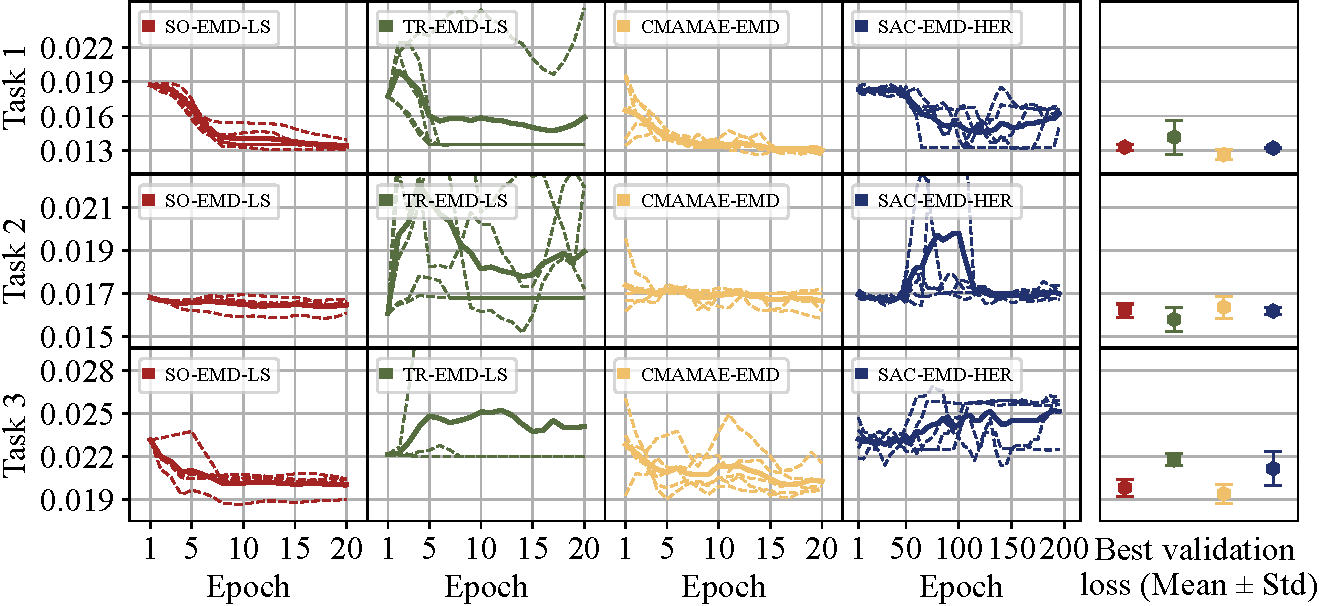
\includegraphics[width=\columnwidth]{images/task_baseline.pdf}
    \caption{Performances achieved by different methods on soil digging tasks with demonstrations. SO: gradient-based skill optimisation. LS: line search. TR: gradient-based trajectory optimisation. CMAMAE: Covariance Matrix Adaptation MAP-Annealing. SAC: soft actor-critic. HER: hindsight experience replay.}\label{subfig:task-baseline}
    \end{subfigure}\\
    \begin{subfigure}{0.6\columnwidth}
        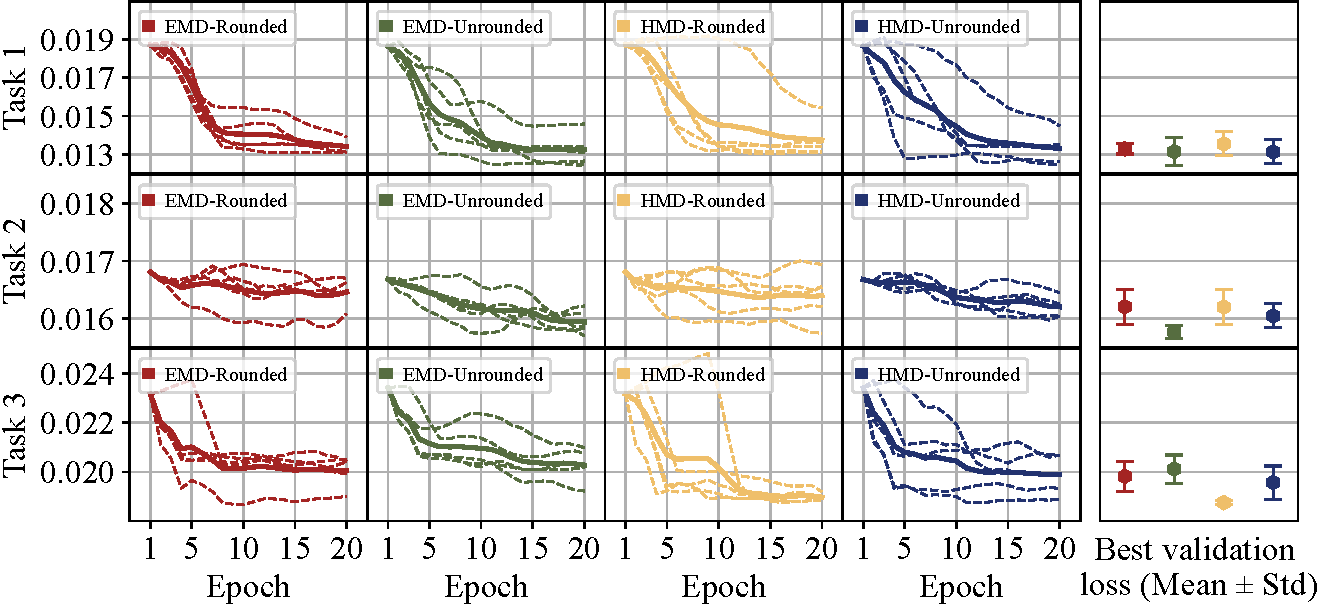
\includegraphics[width=\columnwidth]{images/task_soil_rg.pdf}
    \caption{Gradient-based skill optimisation (with line search) ablation on using the unrounded number of timesteps in the skill-to-action mapping.}\label{subfig:task-rg}
    \end{subfigure}
\caption{Validation losses for baselines and ablation. Validation loss: the sum of the EMD and HMD loss averaged over the sampling resolution ($40\times40$). EMD: Earth mover's distance. HMD: height map distance.}\label{fig:task-bl-ab}
\end{figure}

\end{adjustwidth}

\end{reply}

%=========================================%
% Begin a new reviewer section
\clearpage
\reviewersection
%-----------------------------------------%
\begin{point}
1. The contributions of this article should be summarized. The current version looks like a list of work. 
\end{point}

\begin{reply}
\noindent\rp{Dear reviewer 1, thanks for the insightful comment. We have made significant modifications in the abstract, introduction and conclusion sections to better reflect the core contributions of this article. They are quoted as follows.}

\begin{adjustwidth}{20pt}{20pt}
\vspace{0.3cm}\noindent\xt{\textbf{Abstract} (Page 1)}

Automating the manipulation of granular materials poses significant challenges due to complex contact dynamics, unpredictable material properties, and intricate system states. Existing approaches often fail to achieve efficiency and accuracy in such tasks. To fill the research gap, this paper \xt{studies the small-scale and high-precision granular material digging task with unknown physical properties. A new framework, named differentiable digging robot (DDBot), is proposed to manipulate granular materials, including sand and soil.}

\xt{Specifically, we equip DDBot with a differentiable physics-based simulator, tailored for granular material manipulation, powered by GPU-accelerated parallel computing and automatic differentiation. DDBot can perform efficient differentiable system identification and high-precision digging skill optimisation for unknown granular materials, which is enabled by a differentiable skill-to-action mapping, a task-oriented demonstration method, gradient clipping and line search-based gradient descent.}

\xt{Experimental results show that DDBot can efficiently (converge within $5$ to $20$ minutes) identify unknown granular material dynamics and optimise digging skills, with high-precision results in zero-shot real-world deployments, highlighting its practicality. Benchmark results against state-of-the-art baselines also confirm the robustness and efficiency of DDBot in such digging tasks.}

\vspace{0.3cm}\noindent\xt{\textbf{Introduction} (Page 2, left column, paragraphs 2 to 4)}

\xt{...}

\xt{To fill the research gap, this article makes the following contributions to the robotisation of real-world, small-scale and high-precision granular material digging tasks with unknown material properties.}

\xt{First, to the best of our knowledge, this is the first attempt to develop an efficient and high-fidelity differentiable simulator specifically designed for granular material manipulation. It supports efficient forward dynamics computation to train data-driven methods, such as DRL, and evaluate non-learning methods, such as MPC. It also enables efficient automatic differentiation to support gradient-based optimisation methods, such as RMSProp~\cite{tieleman2012rmsprop}.}

\xt{Secondly, based on the proposed simulator, we present a novel framework, named differentiable digging robot (DDBot) (Figure 1), which allows first-order gradient-based optimisation in system identification tasks and small-scale high-precision digging tasks for real-world granular materials with unknown properties.We experimentally show that gradient-clipping is effective in stopping gradient explosion in SVK and DP-based granular dynamics.} 

\xt{DDBot uses a differentiable digging skill to significantly reduce the solution space and improve manipulation quality, initialises manipulation solution before optimisation via target-oriented demonstrations to accelerate convergence, and performs line search-based gradient descent with adaptive step sizes to stabilise convergence.}

\xt{Last, we experimentally confirm the feasibility of differentiable system identification with soil and sand materials. For digging skill optimisation, we evaluate and benchmark, for the first time, the performances on a series of soil and sand digging tasks with state-of-the-art manipulation optimisation methods, confirming the robustness and efficiency of our DDBot system. Evaluation on a real-world UR5 robot arm is performed to confirm the practicality of the optimised digging motions.}

\xt{...}

\vspace{0.3cm}\noindent\xt{\textbf{Conclusions} (Page 16)}

\xt{Granular material manipulation is of high importance to many real-world scenarios, but the field significantly lacks research and engineering experiences, particularly in small-scale and high-precision manipulation tasks with unknown material properties.} This work thereby studied the challenging real-world granular material manipulation problem with unknown material properties in the context of \textit{small-scale and high-precision} digging. \xt{A differentiable digging robot (DDBot) system was developed for solving such manipulation tasks using a differentiable physics (DP) simulator and a first-order gradient-based optimisation method (RMSProp). The DP simulator was tailored for granular material manipulation for fast data collection, trajectory evaluation and gradient computation, powered by GPU-accelerated parallel computing and automatic differentiation. A differentiable digging skill was designed to reduce the solution space and improve manipulation motion quality. The issues of exploding and fluctuating gradients were studied and resolved through gradient clipping and line search, enabling gradient-based optimisation. To speed up convergence, a digging target-oriented demonstration method is created to serve as an initial solution or form an explorative data distribution.}

\xt{The quantitative and visualisation results of extensive experiments confirmed that DDBot achieves high-quality system identification and skill optimisation performances with sand and soil materials. The optimised solutions were successfully deployed on a UR5e robotic arm in the real world without any adaptation (zero-shot sim-to-real transfer), achieving high digging precision (location and depth errors $<6$ mm, area error $\sim10.8$ cm$^2$). In addition, with GPU acceleration and the proposed gradient treatments, DDBot achieved nearly practically applicable optimisation efficiency (converges in $5$ minutes with a good initial solution).} 

\xt{The performance of DDBot was benchmarked against gradient-based trajectory optimisation, deep reinforcement learning (pointnet-backboned goal-conditioned soft actor-critic) and model predictive control (covariance matrix adaptation map-annealing). Results showed that trajectory optimisation and reinforcement learning (RL) failed in all tasks, while our method and model predictive control succeeded with comparable performances and efficiency. It was suggested that 1) optimisation in the trajectory space for long-horizon tasks should be avoided whenever possible, and 2) when an efficient and physically realistic simulator is available, DRL methods that learn a neural network are counterproductive, gradient-free methods like CMA-MAE lack considerations of the system dynamics, whereas first-order gradient descent methods are preferred for optimisation in the skill parameter space leveraging the gradients computed through the system dynamics.}

\xt{...}

\end{adjustwidth}

\end{reply}

%-----------------------------------------%
\begin{point}
2.The realated work is not stated enough. The advantages and disadvantages of the current work are not discussed in detail. The most important is to find out limitations of previous work and introduce the motivation. 
\end{point}

\begin{reply}

\rp{Thanks for pointing out the lack of clarity in the related work section. We have revised the relevant texts to better reflect the research gap that our work seeks to address in comparison to the literature. The modified content is quoted below.}

\begin{adjustwidth}{20pt}{20pt}
\vspace{0.3cm}\noindent\xt{\textbf{RELATED WORK} (Page 2, right column)}

\noindent\xt{A. Robotic soil manipulation tasks}

\xt{...}

\xt{The disadvantages of these approaches are primarily twofold. First, they are restricted to a single manipulation motion, inapplicable to ever-changing task requirements and unknown soil properties. Second, they were developed for large-scale operations without the need to satisfy high-precision small-scale control, which is heavily challenged by the difficulty of precisely modelling the physical processes of the materials.
Against this background, we develop a robotic granular material manipulation method that deals with \textit{high-precision} small-scale operations in unstructured environments with \textit{changing task requirements} (varying hole shapes) and \textit{unknown material properties}}.

\xt{...}

\noindent\xt{B. Robotic granular material manipulation methods}

\xt{...}

\xt{In summary, there is no existing approach that targets \textit{high-precision} digging tasks, which are challenged by the difficulty of simulating the high-fidelity dynamics of the target granular material with \textit{unknown properties}. This paper fills this gap by studying such tasks. Method-wise, existing approaches are inefficient with high-fidelity physics dynamics and have to trade off manipulation precision to increase computation efficiency. On the contrary, our novel gradient-based digging skill optimisation method can maintain both high manipulation precision and computational efficiency through a GPU-accelerated parallel computing-supported simulator.}

\xt{...}

\end{adjustwidth}

\end{reply}

%-----------------------------------------%
\begin{point}
3.The reviewer thinks the system dynamics should be modeled as the
equation. Is it used to build the trainning environment? 
\end{point}

\begin{reply}
\rp{Thanks for the valuable comment. We agree that this would add to the clarity of the article and have included some more details of the dynamic model in the method section. Mainly, we provide more details of the key equations of the constitutive models governing the elastic and plastic deformation behaviours. The new content is quoted below.}

\begin{adjustwidth}{20pt}{20pt}
\vspace{0.3cm}\noindent\xt{\textbf{METHOD} (Page 5, Section III-A, left column, paragraph 2)}

\xt{For the sake of clarity, we present the key equations of the constitutive models (hyperelasticity and plasticity) and a simplified procedure of MLS-MPM below. Please refer to~\cite{klar2016drucker} for a complete illustration of the dynamic model. As an explicit simulation algorithm, MLS-MPM advances simulation time in a global/local time-stepping process~\cite{hu2018moving}. In other words, for the $t$-th simulation step ($0 < t\leq T$) with a simulation stepsize $\Delta t$, there are $N$ substeps with a sub-stepsize $\Delta t_{sup}=\Delta t / N$. Denote $\pmb{x}^{n+1}_p = f_{sub}^{t,n}(\pmb{x}^n_p, a_t, \pmb{\Theta}, \pmb{g}, \Delta t_{sup})$ as the function of the $n$-th substep of the $t$-th step, it can be summarised as the list of consecutive functions shown in Algorithm 1.}

\xt{In Algorithm 1, line 4, the constitutive model $f_{constitutive}$ first alters the deformation gradient $F^{tmp}_p$ based on the plasticity model for any particle that undergoes plastic deformation. Then it computes the stress of that particle using the altered deformation gradient $F_p'$ and the hyperelasticity energy model. With the singular value decomposition (line 3 of Algorithm 1) of the deformation gradient for particle $p$ after the last iteration update, the SVK elastic energy density function can be written in terms of the diagonal matrix $S_p$:}

\setcounter{equation}{2}
\xt{\begin{equation}\label{eq:SVK}
\psi_p(F) = \mu \mathrm{tr}((\ln S_p)^2) + \frac{1}{2}\lambda \mathrm{tr}((\ln S_p)^2)
\end{equation}}

\noindent \xt{whose derivative is the first Piola–Kirchhoff stress tensor:}

\xt{\begin{equation}\label{eq:piola}
\bm{P}_p = \frac{\partial\psi_p}{\partial F} = U_p\ (2\mu S^{-1}_p\ln S_p + \lambda \mathrm{tr}(\ln S_p)S^{-1}_p)\ V^T_p
\end{equation}}

\noindent \xt{where $\mu$ and $\lambda$ are the Lam\'e constants and can be derived from the Young's modulus $E$ and Poisson's ratio $\nu$:
\begin{equation}
\mu = \frac{E}{2(1+\nu)} \quad \lambda = \frac{E \nu}{(1+\nu)(1-2\nu)}
\end{equation}}

\xt{Plasticity is most conveniently controlled by altering $S_p$. The DP yield criterion states the following. Let $\pmb{\epsilon}_p = \ln S'_p$, and
\begin{equation}
\hat{\pmb{\epsilon}_p} = \pmb{\epsilon}_p - \frac{\mathrm{tr}(\pmb{\epsilon}_p)}{dim} \quad \delta_{\gamma_{p}} = \left\Vert \hat{\pmb{\epsilon}_p} \right\Vert + \frac{\lambda dim+2\mu}{2\mu}\mathrm{tr}(\pmb{\epsilon}_p) \alpha_f
\end{equation}}

\noindent \xt{where $\alpha_f = \sqrt{\frac{2}{3}}\frac{2\sin{\phi_{f}}}{3-\sin{\phi_{f}}}$, $dim$ is the spatial dimension of the problem ($3$ in our case), $\delta_{\gamma_{i}}$ is the amount of plastic deformation, and $\phi_{f}$ is the friction angle of sand/soil. The DP model alters $S_p$ under different conditions as follows:
\begin{equation}
    \hat{S}_p=
    \begin{cases}
    I_{d \times d} \hfill & \mathrm{tr}(\pmb{\epsilon}_p) > 0,\\
    S_p \hfill & \mathrm{tr}(\pmb{\epsilon}_p) \leq 0 \And \delta \gamma_{p} \leq 0, \\
    \exp(\pmb{\epsilon}_p-\delta \gamma_{p}\frac{\hat{\pmb{\epsilon}_p}}{\|\hat{\pmb{\epsilon}_p}\|}) \hfill & \mathrm{tr}(\pmb{\epsilon}_p) \leq 0 \And \delta \gamma_{p} > 0.
    \end{cases}\label{eq:DP}
\end{equation}}

\xt{Please refer to~\cite{klar2016drucker} for details of the three conditions. With $\hat{S}_p$, the deformation gradient after plasticity is $F_p' = U_p \hat{S}_p V^{T}_p$ and the Cauchy stress $\sigma_p = \bm{P}_p'{F'_p}^T$, where $\bm{P}_p'$ is computed by substituting $\hat{S}_p$ into Eq.~\ref{eq:piola}.}

\xt{Given an action (Cartesian space displacement) at time $t$, the 6D Cartesian pose of the manipulation (agent) is updated by evenly distributing the action over the $N$ substeps and adding it to the manipulator pose at each substep (line 7 in Algorithm 1). The collision behaviours between the particles/grid and the manipulator are modelled by a signed distance field-based collision detection mechanism and the Columb frictional contact model, following the practices of previous works~\cite{hu2018moving,xy2024sysid}.}

\end{adjustwidth}

\end{reply}

%-----------------------------------------%
\begin{point}
4.The novelty of the method should be discussed after the method is
introduced. The current version merely point out it is different from
the current methods. The relations between advantages and differences
are not clear.
\end{point}

\begin{reply}
\rp{Thanks for raising this concern about the novelty of the method. As mentioned also in some of the previous replies, we have made significant revisions to state our novelty more clearly. Besides the added contents in the abstract, introduction, related work and conclusion sections quoted above, we add a few sentences at the beginning of the method section also. This is quoted below.}

\begin{adjustwidth}{20pt}{20pt}
\vspace{0.3cm}\noindent\xt{\textbf{METHOD} (Page 3, right column, first paragraph)}

This section presents details of our method for robotic soil/sand digging. An overview of the proposed DDBot system is given in Figure 1. \xt{The primary novelties of the DDBot system are twofold: 1) the use of GPU-accelerated, parallel computing-supported, and MPM-based physics simulation for granular material dynamics that is both time-efficient and physically precise, 2) the complete differentiability of the physics simulator that allows efficient gradient descent algorithms to optimise physics parameters and manipulation skills/trajectories. With the use of gradient-clipping and line search-based gradient update, DDBot can accomplish highly precise granular digging tasks in $5$ minutes. The rest of this section starts by mathematically formalising the digging task and the proposed digging skill, introducing the skill demonstration, discussing the differentiability of the system components, and how to stop gradient explosion and converge over rugged losses.}
\end{adjustwidth}

\end{reply}

\begin{point}
5.The authors claim that studying the feasibility of differentiable
simultaneous skill selection and optimisation is the future research
direction. Why is it challenging to study in the current article.   
\end{point}

\begin{reply}
\rp{Thanks for pointing out the lack of explanation of this statement. We have revised it and elaborated on the subject. The new content is quoted below.}

\begin{adjustwidth}{20pt}{20pt}
\vspace{0.3cm}\noindent\xt{\textbf{CONCLUSION} (Page 16, left column, last paragraph)}

\xt{...}

Currently, the proposed system is limited to a fixed task initiation (soil/sand always flat) and optimising only one skill. This is due to the difficulty of reconstructing 3D scenes involving granular materials with high precision. In the future, integrating an efficient 3D reconstruction module into the DDBot system will facilitate the optimisation of multiple skills. In addition, optimising the order of multiple skills is a discrete optimisation problem. \xt{The gradient of a discrete decision-making process requires careful treatment to enable differentiability (e.g., the Softmax operation). Computing the gradient chain will become combinatorially slow as it branches for multiple skills at every skill selection stage.} Studying the feasibility of differentiable simultaneous skill selection and optimisation \xt{is parallel to many other research topics such as task and motion planning and hierarchical reinforcement learning. A considerable amount of research and engineering effort is needed to develop new algorithms for such tasks in the future.}
\end{adjustwidth}

\end{reply}

%=========================================%
% Begin a new reviewer section
\reviewersection
\textbf{General assessment:} 
This is a complete piece of work that well motivates the benefits of
differentiable physics simulators for robot digging of unknown granular
materials. The problem statement uses POMDP framework, and the main
ingredients can be identified such as gradient-based digging skill
parameter optimization with gradient clipping. The extensive
experimental validation is appreciated. The visualizations and
statistics are convincing. 

\begin{reply}
\rp{Dear Reviewer 2, we are very grateful for your recognition and valuable comments on this paper. Please read below the improvements that your comments have helped to make for this paper.}

\end{reply}

%-----------------------------------------%
\begin{point}
- It is not clear which is the output of algorithm 1. Is the set of
theta params the input? 
\end{point}

\begin{reply}
\rp{Thanks for pointing out the unclear presentation of the algorithm. We have revised the algorithm to show clearly the input and output. The original algorithm 1 has been largely reduced to improve clarity. Please see the new version below.}

\begin{table}[h]
\small
\centering
\begin{tabular}{>{\color{blue}}l}
\toprule
\textbf{Algorithm 2}: Skill-to-action mapping $\bar{a}(\pmb{\theta})=\{a_0,..,a_T\}$\\
\midrule
Inputs: $\theta_{ displace},\theta_{ rotate},\theta_{ insert\_dist},\theta_{ push\_dist},\theta_{ push\_angle}$\\
$d_{ lift}, v_l,v_w,\Delta t$. \\
Output: $\bar{a}=\{a_0,a_1,...,a_T\}$\\
\midrule
With Eqs.~\ref{eq:d1} to~\ref{eq:delta_d4}, Compute: \\
$T_1$, $T_2$, $T_3$, $T_4$, $\Delta x_1$, $\Delta rx_1$, $\Delta x_2$, $\Delta z_2$, $\Delta x_3$, $\Delta z_3$, $\Delta rx_4$, $\Delta z_4$\\
Let $T =T_1+T_2+T_3+T_4$\\
For $t$ from $0$ to $T$: \hspace{0.73cm} $a_t = [0.0, 0.0, 0.0, 0.0, 0.0, 0.0]$\\
For $t$ from $0$ to $T_1-1$: \hspace{0.07cm} $a_t[0] = \Delta x_1$, $a_t[3]=\Delta rx_1$\\
For $t$ from $T_1$ to $T_2-1$: $a_t[0] = \Delta x_2$, $a_t[2]=\Delta z_2$\\
For $t$ from $T_2$ to $T_3-1$: $a_t[0] = \Delta x_3$, $a_t[2]=\Delta z_3$\\
For $t$ from $T_3$ to $T_4-1$: $a_t[3] = \Delta rx_4$, $a_t[2]=\Delta z_4$\\
\bottomrule
\end{tabular}
\end{table}

\end{reply}

%-----------------------------------------%
\begin{point}
It is suggested to better describe the skill optimization problem
introduces in Section III.D. It contains many symbols in the current
notation that are not explicitly mentioned. After algorithm 2, the
chain rule is applied to compute the nabla theta. The last term is the
partial derivative of action w.r.t. theta. Thus, algorithm 1 should be
differentiated or how does this term is computed?

\end{point}

\begin{reply}

\rp{Thanks for pointing out the lack of clarity in presenting the skill optimisation problem. We have added the missing definitions of the symbols and included new statements to clarify or reference the definitions from other places in the article. Please examine section III-D starting from the right column of page 7 to see the added contents in blue.}

\rp{In addition, we have provided the full differentiation results of the skill-to-action mapping. The results are presented at the end of section III-B, with a full derivation process provided in Appendix A. Please examine the second half of Section III-B, starting from page 6, left column, after the definition of the four phases of the digging skill.}

\end{reply}

%=========================================%
% Begin a new reviewer section
\reviewersection
\textbf{General assessment:} 
The paper presents a DDBot framework for digging in granular materials
with unknown properties. First, a gradient-based algorithm with
regularization techniques is introduced to tackle the issue of the
gradient explosion. Then, a differentiable skill-to-action mapping is
established to optimize gradient-based skill. Finally, experiments are
conducted to verify the effectiveness of the proposed schemes.
Theoretically, this study lacks innovation and merely applies existing
optimization techniques to prevent gradient explosion. Experimentally,
this study does not propose a method for evaluating the quality of the
digging task (e.g., if the goal is to dig a circular hole, there is
little assessment of the discrepancy between the final hole created by
the robotic arm and the target hole to validate the effectiveness of
the proposed method). So, I could not recommend acceptance.

\begin{reply}
\rp{Dear Reviewer 3, we are very grateful for your concern for the novelty and presentation of the previous manuscript. We have made extensive changes in the new version in accordance with your comments. We believe that the new manuscript has been much improved with your help. Please examine our responses to your comments below.}
\end{reply}

%-----------------------------------------%
\begin{point}
In Fig. 1, what do the figures generated by real-world digging
manipulation or differentiable physics simulation mean?
\end{point}

\begin{reply}
\rp{Thanks for pointing out the unclear presentation of the figure images. We have included a statement to clarify that} \xt{"The five small images visualise a real-world digging trajectory that matches the trajectory optimised in simulation shown in the green box."}

\end{reply}

%-----------------------------------------%
\begin{point}
In the description of action, what are $\delta x, \delta y, \delta z, \delta a, \delta b$, and $\delta c$?

\end{point}

\begin{reply}
\rp{Thanks for noticing the lack of symbol definitions. They are now formally defined as follow.}

\begin{adjustwidth}{20pt}{20pt}
\vspace{0.3cm}\noindent\xt{\textbf{METHOD} (Page 4, right column, second paragraph)}

\xt{...}

\textbf{Actions:} An action of the robot manipulator at each step here is a 6D displacement vector in the Cartesian space (i.e., end-effector tip frame) $a=[\Delta x, \Delta y, \Delta z, \Delta a, \Delta b, \Delta c]\in\mathcal{A}\subset\mathbb{R}^6$, \xt{i.e., it controls the amount of translational changes in the $x$, $y$, $z$ directions and the rotational changes about these three axes...}

\xt{...}

\end{adjustwidth}

\end{reply}

%-----------------------------------------%
\begin{point}
Algorithm 1 is too lengthy. The authors should simplify it.
Moreover, Algorithm 2 is unnecessary.
\end{point}

\begin{reply}
\rp{Thanks for raising this concern about the presentation of the algorithms. We have made extensive changes to the presentation of the original algorithm 1, which is now algorithm 2. We have defined more formally the four phases of the digging skill with equations instead of in the algorithm table. The original algorithm 1 is largely implied and now only presents the assembly of the four phases of digging motions into an action trajectory. On the other hand, we agree that the original algorithm 2 is unnecessary and has been removed. Please examine the following contents.}

\begin{adjustwidth}{20pt}{20pt}
    \vspace{0.3cm}\noindent\xt{\textbf{Method} (Section III-B, Page 5)}

\xt{...}

\xt{The skill comprises four phases graphically illustrated by Fig. 2 and mathematically defined by Eqs. 8 to 22, with a list of notations comprised in Table 1. Algorithm 2 presents the assembly of the calculated end-effector displacements into the complete trajectory $\bar{a}(\pmb{\theta})$.}

\begin{table}[h]
\small
\centering
\begin{tabular}{>{\color{blue}}l}
\toprule
\textbf{Algorithm 2}: Skill-to-action mapping $\bar{a}(\pmb{\theta})=\{a_0,..,a_T\}$\\
\midrule
Inputs: $\theta_{ displace},\theta_{ rotate},\theta_{ insert\_dist},\theta_{ push\_dist},\theta_{ push\_angle}$\\
$d_{ lift}, v_l,v_w,\Delta t$. \\
Output: $\bar{a}=\{a_0,a_1,...,a_T\}$\\
\midrule
With Eqs.~\ref{eq:d1} to~\ref{eq:delta_d4}, Compute: \\
$T_1$, $T_2$, $T_3$, $T_4$, $\Delta x_1$, $\Delta rx_1$, $\Delta x_2$, $\Delta z_2$, $\Delta x_3$, $\Delta z_3$, $\Delta rx_4$, $\Delta z_4$\\
Let $T =T_1+T_2+T_3+T_4$\\
For $t$ from $0$ to $T$: \hspace{0.73cm} $a_t = [0.0, 0.0, 0.0, 0.0, 0.0, 0.0]$\\
For $t$ from $0$ to $T_1-1$: \hspace{0.07cm} $a_t[0] = \Delta x_1$, $a_t[3]=\Delta rx_1$\\
For $t$ from $T_1$ to $T_2-1$: $a_t[0] = \Delta x_2$, $a_t[2]=\Delta z_2$\\
For $t$ from $T_2$ to $T_3-1$: $a_t[0] = \Delta x_3$, $a_t[2]=\Delta z_3$\\
For $t$ from $T_3$ to $T_4-1$: $a_t[3] = \Delta rx_4$, $a_t[2]=\Delta z_4$\\
\bottomrule
\end{tabular}
\end{table}

\xt{\textbf{Phase 1:} moving the shovel in the world's $x$ axis by a distance $d_1$ and rotating about the shovel's $x$ axis by an angle $\varphi_1$. Eqs.~\ref{eq:d1} to ~\ref{eq:delta_d1} define the calculation of the actions for phase 1 from $\theta_{displace}$ and $\theta_{rotate}$.}

\setcounter{equation}{7}
\begingroup\makeatletter\def\f@size{8}\check@mathfonts\xt{\vspace{-0.3cm}
\begin{flalign}
    &d_1 = \theta_{displace} \cdot 0.12, &&\varphi_1 = \theta_{rotate} \cdot \pi / 3&&&\label{eq:d1}\\
    &T^{float}_{d_1} = |d_1 / (v_l\cdot\Delta t)|, &&T^{float}_{\varphi_1} = |\varphi_1/(v_w\cdot\Delta t)|&&&\label{eq:Tf1}\\
    &T^{float}_1=max(T^{float}_{d_1}, T^{float}_{\varphi_1}), &&T_1 = round(T^{float}_1)&&&\label{eq:Ti1}\\
    &\Delta x_1 = \begin{cases}
        \frac{d_1}{T_1},\ T_1>0\\
        0,\  T_1=0
        \end{cases}\hspace{-0.4cm},
    &&\Delta rx_1 = \begin{cases}
        \frac{\varphi_1}{T_1},\ T_1>0\\
        0,\  T_1=0
        \end{cases}\label{eq:delta_d1}
\end{flalign}}
\endgroup

\xt{\textbf{Phase 2:} inserting the shovel into the soil/sand by a distance $d_2$ along its pointing direction. Eqs.~\ref{eq:d2} to ~\ref{eq:delta_d2} define the calculation of the actions for phase 2 from $\theta_{rotate}$ and $\theta_{insert\_dist}$.}

\begingroup\makeatletter\def\f@size{8}\check@mathfonts\xt{\vspace{-0.3cm}
\begin{flalign}
    &d_2 = (\theta_{insert\_dist}+1)\cdot0.03,\ \varphi_2 = \varphi_1 + \pi /2 &&\label{eq:d2}\\
    &T^{float}_2 = d_2 / (v_l\cdot\Delta t)\label{eq:Tf2}\\
    &T_2 = round(T^{float}_2)\label{eq:Ti2}\\
    &\Delta x_2 = \begin{cases}
        \frac{d_2 \cdot \cos(\varphi_{2})}{T_2},\ T_2>0\\
        0,\  T_2=0
        \end{cases},\ 
    \Delta z_2 = \begin{cases}
        \frac{-d_2 \cdot \sin(\varphi_{2})}{T_2},\ T_2>0\\
        0,\  T_2=0
        \end{cases}\hspace{-1cm}&&\label{eq:delta_d2}
\end{flalign}}
\endgroup

\xt{\textbf{Phase 3:} pushing towards an angle $\varphi_3$ by a distance $d_3$. Eqs.~\ref{eq:d3} to~\ref{eq:delta_d3} define the calculation of the actions for phase 3 from $\theta_{push\_dist}$ and $\theta_{push\_angle}$}.
\begingroup\makeatletter\def\f@size{8}\check@mathfonts\xt{\vspace{-0.3cm}
\begin{flalign}
    &d_3 = (\theta_{push\_dist} + 1) \cdot 0.1 + 0.04,\ \varphi_3 = (\theta_{push\_angle} + 3) \cdot \pi /3\hspace{-0.4cm}&&\label{eq:d3}\\
    &T^{float}_3 = |d_3 / (v_l\cdot\Delta t)|&&\label{eq:Tf3}\\
    &T_3 = round(T^{float}_3)&&\label{eq:Ti3}\\
    &\Delta x_3 = \begin{cases}
        \frac{d_3 \cdot \cos(\varphi_3)}{T_3},\ T_3>0\\
        0,\  T_3=0
        \end{cases},\
    \Delta z_3 = \begin{cases}
        \frac{d_3 \cdot \sin(\varphi_3)}{T_3},\ T_3>0\\
        0,\  T_3=0
        \end{cases}\hspace{-1cm}&&\label{eq:delta_d3}
\end{flalign}}
\endgroup

\xt{\textbf{Phase 4:} rotating back to straight and lifting for a constant distance $d_4=0.01$ m. Eqs.~\ref{eq:Tf4} to~\ref{eq:delta_d4} define the calculation of actions for phase 4.}
\begingroup\makeatletter\def\f@size{8}\check@mathfonts\xt{\vspace{-0.3cm}
\begin{flalign}
    &T^{float}_{d_4} = d_4 / (v_l\cdot\Delta t) &&&\label{eq:Tf4}\\
    &T^{float}_4 = max(T^{float}_{\varphi_1}, T^{float}_{lift}), &&T_4 = round(T^{float}_4)&&&\label{eq:Ti4}\\
    &\Delta rx_4 = \frac{- \varphi_1}{T_4},&&\Delta z_4 = \frac{d_4}{T_4}&&&\label{eq:delta_d4}
\end{flalign}}
\endgroup

\xt{...}
\end{adjustwidth}

\end{reply}

%-----------------------------------------%
\begin{point}
Appendix A, given by the authors, is about the SVK and DP
model, which are not the contributions of this study. The authors
should delete it.
\end{point}

\begin{reply}
\rp{Thanks for the important advice. We agree that this part is not the contribution of the study. However, one of the other reviewers has requested that the system dynamics be modelled as equations in the main text. Therefore, we have moved part of the original Appendix A (now Appendix B) to the method section. This gives the reader a bit more information about the system dynamics. In addition, we argue that the differentiation proof is of importance to show that these two models are indeed differentiable towards the physical parameters of the materials. Therefore, we reduced the content in the original Appendix A as a compromise to all reviewers and kept minimal information required to provide readers with the necessary information.}

\end{reply}

%-----------------------------------------%
\begin{point}
Many notations, such as dim(), are not interpreted in this
paper. The authors should add a notation table to clarify it.
\end{point}

\begin{reply}
\rp{Thanks for the comment. We have added the meaning of the symbols and included a notation table for them in the method section.}

\end{reply}

%-----------------------------------------%
\begin{point}
Fig. 5 exhibits the role of the three regularization techniques
“introduced” by the authors. So, Fig. 5 is unnecessary, and the authors
should pick the most efficient technique, which should not be listed as
a contribution of this paper.
\end{point}

\begin{reply}
\rp{Thanks for pointing out the lack of clarity in claiming the contributions in the previous manuscript. Indeed, we agree that the original Fig. 5 adds little value and has been moved to Appendix C. We also made considerable revisions to better reflect the contribution of the article. We apologise for the confusing wording that was used in the previous manuscript. We agree that the gradient regularisation techniques themselves have been adopted in other research and engineering practices for decades. However, their effectiveness has not been studied in the context of differentiable physics simulation, especially not for granular material manipulation tasks modelled by the St. Venant-Kirchoff (SVK) elastic energy and the Drucker-Prager (DP) plastic yield criterion. We have made modifications to highlight the experimental novelty in the investigation of the gradient instability issues and the effects of the techniques, instead of their theoretical development. Below are the key relevant changes.}

\begin{adjustwidth}{20pt}{20pt}

% \vspace{0.3cm}\noindent\xt{\textbf{Abstract} (Page 1)}

% \xt{... The issues of gradient explosion and fluctuation are investigated and resolved through gradient clipping and line search-based gradient descent...}

\vspace{0.3cm}\noindent\xt{\textbf{Introduction} (Page 2, left column, paragraphs 2 to 4)}

\xt{...}

\xt{... We experimentally show that gradient-clipping is effective in stopping gradient explosion in SVK and DP-based granular dynamics...}

\xt{...}


\vspace{0.3cm}\noindent\xt{\textbf{Method} (Section III-E, Page 8, left column, last paragraph)}

\xt{...}

We \xt{experiment on} three techniques to regularise the scale of the gradient for key variables in the MLS-MPM algorithm, namely \textit{clipping, dynamic-scaling, and normalisation}.

\xt{...}

\vspace{0.3cm}\noindent\xt{\textbf{Conclusions} (Page 16)}

\xt{... The issues of exploding and fluctuating gradients were studied and resolved through gradient clipping and line search, enabling gradient-based optimisation...}

\xt{...}

\end{adjustwidth}

\end{reply}

%-----------------------------------------%
\begin{point}
In experiments, the authors should illustrate how to identify
the performance of the digging task.
\end{point}

\begin{reply}

\rp{Thanks for noticing the insufficient objective measures for a more intuitive understanding of the digging task performances. To address this, we calculated the location, depth and surface area of the target holes and compared them to the measurement of the holes dug by the optimised motions. These statistics have been included in the results. They are quoted below.}

\begin{adjustwidth}{20pt}{20pt}
\vspace{0.3cm}\noindent\xt{\textbf{RESULTS - DIGGING TASKS} (Section VII, Page 13, last paragraph of the section and Table IV)}

\xt{...}

\xt{...To statistically evaluate the performance, we calculate the centres, depths and areas of the real-world dug holes using their height maps. Table IV compares these statistics of the task targets and the holes dug by the best skill found by our method. It was found that, over the six tasks, the average difference in hole centres is no more than $6$ mm, the average difference in hole depth is $2.5$ mm, and the average area difference is $10.8$ cm$^2$...}

\setcounter{table}{3}
\begin{table}[h]
\centering
\begin{tabular}{ABCDDD}
\toprule
\textbf{Features} (cm)          &                       &         & \textbf{Task 1} & \textbf{Task 2} & \textbf{Task 3} \\
\midrule
                                & \multirow{2}{*}{Soil} & Targets & (6.79, -0.08) & (-6.23, 0.03) & (3.12, -0.97)\\
\textbf{Center}                 &                       & Results & (5.61, -0.52) & (-6.73, -0.65)& (3.27, -0.64)\\
\cline{2-6}
\textbf{(x, y)}                 & \multirow{2}{*}{Sand} & Targets & (6.60, -0.15) & (-2.58, 0.17) & (8.57, 0.18)\\
                                &                       & Results & (5.92, -0.63) & (-4.11, -0.51) & (8.85, -0.86)\\
\midrule
\multirow{4}{*}{\textbf{Depth}} & \multirow{2}{*}{Soil} & Targets & 1.74   & 1.48   & 2.43 \\
                                &                       & Results & 1.69   & 1.48   & 2.78 \\ 
\cline{2-6}
                                & \multirow{2}{*}{Sand} & Targets & 0.74   & 1.75   & 1.48\\
                                &                       & Results & 1.18   & 1.38   & 1.76\\
\midrule
\multirow{4}{*}{\textbf{Area}}  & \multirow{2}{*}{Soil} & Targets & 24.84  & 27.72  & 46.80 \\
                                &                       & Results & 24.12  & 32.04  & 78.48\\ 
\cline{2-6}
                                & \multirow{2}{*}{Sand} & Targets & 17.28  & 52.20  & 50.40 \\
                                &                       & Results & 30.96  & 52.20  & 46.08\\
\bottomrule
\end{tabular}
\caption{\xt{Statistics of the real-world dug holes (cm). The averaged differences of hole centre, depth and area across the six tasks are (0.60, 0.59) cm, 0.25 cm and 10.8 cm$^2$.}}
\label{tab:holes}
\end{table}

\end{adjustwidth}
\end{reply}
\printbibliography

\end{document}